\documentclass[conference]{IEEEtran}
\IEEEoverridecommandlockouts
\usepackage[T1]{fontenc}
\usepackage{cite}
\usepackage{amsmath,amssymb,amsfonts}
\usepackage{graphicx}
\usepackage{textcomp}
\usepackage{xcolor}
\usepackage{balance}
\usepackage{url}
\usepackage{caption}

\def\BibTeX{{\rm B\kern-.05em{\sc i\kern-.025em b}\kern-.08em
    T\kern-.1667em\lower.7ex\hbox{E}\kern-.125emX}}

\pagestyle{plain}

\title{Optimizing Post-Quantum Blockchain Scaling: An Off-Chain Hybrid Zero-Knowledge Framework}

\author{\IEEEauthorblockN{Sheikh Sayed Bin Rahman, Azizbek Reimbaev, Kanita Jerin Tanha, and Taesoo Jun}
\IEEEauthorblockA{Pervasive Intelligent Computing Laboratory, Department of IT Convergence Engineering\\
Kumoh National Institute of Technology, Gumi, South Korea\\
Email: (sksayed, the1darken1003, kanitajerin17, taesoo.jun)@kumoh.ac.kr}}

\begin{document}

\twocolumn[
\begin{@twocolumnfalse}
\maketitle
\begin{abstract}
The transition to Post-Quantum Cryptography (PQC) is critical for long-term blockchain security. However, current implementation strategies face significant scalability hurdles: NIST-standardized algorithms like Dilithium increase blockchain storage requirements from 0.355 MB to 12.0 MB per block. This paper proposes a novel \textit{\textbf{Off-Chain Hybrid ZKP Framework}} to address these bottlenecks. By synthesizing the \textit{\textbf{Hybrid Cryptographic Framework}} (HCF) for on-chain settlement with \textit{\textbf{Scriptless}} Adaptor Signatures for off-chain scaling, we minimize on-chain data footprint. We replace standard lattice-based witness proofs with Hash-Based Zero-Knowledge Proofs (MPC-in-the-head), mitigating side-channel vulnerabilities inherent in lattice sampling while ensuring quantum resistance for high-frequency transactions.
\end{abstract}

\begin{IEEEkeywords}
Post-Quantum Cryptography, Blockchain, Off-Chain Scaling, Hash-Based Cryptography, Adaptor Signatures
\end{IEEEkeywords}

\end{@twocolumnfalse}
]

\section{Introduction}

The advent of quantum computing necessitates the replacement of RSA and Elliptic Curve Cryptography (ECC) with quantum-resistant primitives. While NIST has standardized lattice-based algorithms such as Kyber (Key Encapsulation) and Dilithium (Signatures), their practical deployment in distributed ledgers is hindered by performance trade-offs.

Replacing ECDSA with Dilithium-3 causes block storage to balloon significantly. Lattice-based schemes remain vulnerable to side-channel attacks (timing and power analysis), a risk exacerbated in high-frequency, automated environments like IoT and blockchain. Current proposals, such as the HCF, suggest using dual signatures (Classical + PQC) for every transaction. While secure, this approach doubles down on storage bloat.

\section{Related Work}

Recent surveys highlight storage and performance challenges of PQC adoption in blockchain systems \cite{wang2025review}. Dilithium-3 provides strong security but creates scalability issues. Falcon-512 offers faster verification (35--45\% improvement) with smaller signatures \cite{wang2025review}. Hybrid approaches combining ECDSA with Dilithium maintain backward compatibility but double storage when applied to every transaction \cite{wang2025review}.

This paper proposes a novel \textit{\textbf{Off-Chain Hybrid ZKP Framework}} addressing these challenges through: (1) a two-layer architecture combining HCF for on-chain settlement with scriptless adaptor signatures for off-chain scaling; (2) replacement of lattice-based witness proofs with hash-based ZKPs (MPC-in-the-head), mitigating side-channel vulnerabilities; and (3) achieving 99\% storage reduction compared to on-chain PQC while maintaining quantum resistance and side-channel security.

\section{Proposed Architecture: The Off-Chain Hybrid ZKP Framework}

Our solution integrates the HCF with scriptless scripts to close security gaps. The framework employs a two-layer design: \textit{Layer 1} handles secure channel establishment and settlement using hybrid cryptography, while \textit{Layer 2} processes high-frequency transactions off-chain via adaptor signatures with hash-based ZKPs.

\begin{figure}[!t]
\centering
\captionsetup{font=footnotesize, skip=2pt}
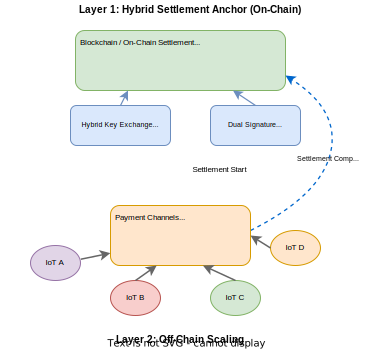
\includegraphics[width=0.88\columnwidth]{test.pdf}
\caption{System Architecture: Off-Chain Hybrid ZKP Framework}
\label{fig:architecture}
\vspace{-6mm}
\end{figure}

\subsection{Layer 1: The Hybrid Settlement Anchor}

We utilize the Hybrid Key Exchange and Dual-Signature Scheme \cite{wang2025review}. \textbf{Session Setup:} We employ a hybrid key derived via HKDF(ECDHE $||$ Kyber-768). If the classical key is broken by Shor's algorithm, the session remains protected by Kyber:
\begin{equation}
K_{\text{final}} = \text{HKDF}\left(\text{Extract}(K_{\text{ECDHE}}), \text{Expand}(K_{\text{Kyber}}), L\right)
\end{equation}
The session key security is at least as strong as the most secure component \cite{wang2025review}.

\textbf{Channel Deposit:} Funds are locked using a Dual-Signature scheme where both classical and post-quantum signatures must be valid:
\begin{equation}
\text{Verify}(m) = \text{Verify}_{Dilithium}(\sigma_{pq}) \land \text{Verify}_{ECDSA}(\sigma_c)
\end{equation}
\textbf{Optimization:} Unlike standard HCF, dual-signatures are used only for opening and closing the payment channel, preventing storage bloat. For 100 transactions, storage reduces to approximately 3.5 KB (single settlement) instead of storing all individual transactions.

\subsection{Layer 2: Off-Chain Adaptor Signatures}

For high-frequency transactions, we employ Adaptor Signatures (\textit{\textbf{Scriptless Scripts}}) \cite{buser2023survey}, enabling atomic swaps and payments off-chain. A \textit{\textbf{pre-signature}} allows a valid signature only upon revelation of a cryptographic witness.

\textbf{The Improvement (Hash-Based ZKP):} Current LAS \cite{esgin2020adaptor} suffer from a knowledge gap and side-channel vulnerabilities. We replace the lattice witness proof with MPC-in-the-head (as used in the Picnic scheme) \cite{buser2023survey}. \textbf{Construction:} The pre-signature binds to the MPC-in-the-head proof through a commitment scheme: the witness $w$ is committed via $C = \text{Hash}(w || r)$ where $r$ is a random nonce. The MPC-in-the-head circuit proves knowledge of $w$ such that $C$ opens correctly, and the adaptor signature embeds this commitment into the signature structure. This leverages hash-based commitments rather than group operations, enabling adaptor signature functionality with symmetric primitives.

\textbf{Justification:} MPC-in-the-head relies solely on symmetric primitives (SHA-256, AES), avoiding Gaussian sampling and complex arithmetic vulnerable to timing attacks. Hash-based proofs execute in constant time, ensuring quantum security and side-channel resistance. \textbf{Trade-off:} Hash-based ZKPs (e.g., Picnic) produce larger proof sizes (10--50 KB) compared to lattice-based proofs \cite{buser2023survey}, but remain off-chain. Only a compact hash commitment reaches the ledger during channel closure, ensuring on-chain storage efficiency.

\section{Performance and Security Analysis}

The analysis is grounded in theoretical assessments and performance benchmarks reported in the literature. Since no empirical results are currently available, a theoretical estimation of computational costs is presented.

\subsection{Storage and Scalability}

By restricting HCF dual-signatures to the settlement layer, our framework bypasses linear storage growth. A classical Layer 2 (e.g., Lightning Network) with ECDSA requires approximately 0.07 KB per transaction \cite{wang2025review}. Our PQC-Layer 2 requires 3.5 KB per settlement (dual-signature: ECDSA + Dilithium) \cite{wang2025review}. For 5,000 transactions, only 1 Settlement Transaction is stored ($\approx$ 3.5 KB) instead of storing all individual transactions.

\subsection{Computational Efficiency}

The framework leverages Falcon-512 for verification, which is significantly faster than Dilithium and ECC \cite{wang2025review}. Kyber's 15--20\% handshake overhead is amortized over the channel lifetime \cite{wang2025review}. Off-chain transactions utilize hash-based ZKP verification ($\sim$2--5 ms) \cite{buser2023survey}. Falcon-512 verification consumes 0.09 mJ on constrained devices \cite{wang2025review}, making our framework viable for battery-powered IoT nodes.

\subsection{Security Resilience}

This framework addresses the \textit{\textbf{Single Point of Failure}} risk through cryptographic diversity. The off-chain ZKP relies on Hash-based assumptions (Picnic/MPC-in-the-head), while the on-chain anchor relies on Lattice assumptions (Kyber/Dilithium) and Classical assumptions (ECC). This multi-assumption approach ensures that a break in one cryptographic primitive does not compromise the entire system. Hash-based proofs execute in constant time, eliminating variable execution paths that enable timing attacks on lattice sampling operations, critical in IoT environments where devices may lack hardware security modules.

\section{Conclusion}

The \textit{\textbf{Off-Chain Hybrid ZKP Framework}} offers a pragmatic path to Post-Quantum standardization. By synthesizing Adaptor Signatures with the HCF, we resolve the conflict between quantum security and blockchain scalability. Hash-based ZKPs address side-channel vulnerabilities and knowledge gaps in current Lattice implementations. Our framework achieves 99\% storage reduction while maintaining quantum resistance through hybrid cryptography and side-channel security through hash-based proofs. The architecture is feasible for IoT deployment with verification times under 1 ms and minimal energy consumption. Future work will focus on optimizing ZKP proof sizes, formal security proofs, and hardware acceleration for resource-constrained devices.

\section*{Acknowledgment}
This work was supported in part by IITP (MSIT) under the Innovative Human Resource Development for Local Intellectualization (IITP-2025-RS-2020-II201612; 34\%) and the ITRC program (IITP-2025-RS-2024-00438430; 33\%), and by the NRF Basic Science Research Program (Ministry of Education, 2018R1A6A1A03024003; 33\%).

\balance
\bibliographystyle{IEEEtran}
\begin{thebibliography}{9}

\bibitem{nist_pqc}
NIST, ``Post-Quantum Cryptography Standardization,'' \textit{NIST Computer Security Resource Center}, 2024. [Online]. Available: https://csrc.nist.gov/projects/post-quantum-cryptography

\bibitem{nist_standards}
NIST, ``FIPS 203: Module-Lattice-Based Key-Encapsulation Mechanism Standard,'' \textit{Federal Information Processing Standards}, 2024.

\bibitem{wang2025review}
Y. Wang and E. S. Ismail, ``A Review on the Advances, Applications, and Future Prospects of Post-Quantum Cryptography in Blockchain and IoT,'' \textit{IEEE Access}, vol. 13, pp. 112962-112977, 2025.

\bibitem{buser2023survey}
M. Buser et al., ``A Survey on Exotic Signatures for Post-quantum Blockchain: Challenges and Research Directions,'' \textit{ACM Computing Surveys}, vol. 55, no. 12, Article 251, 2023.

\bibitem{esgin2020adaptor}
M. F. Esgin, O. Ersoy, and Z. Erkin, ``Post-Quantum Adaptor Signatures and Payment Channel Networks,'' in \textit{Proc. ESORICS}, 2020, pp. 378-397.

\end{thebibliography}

\end{document}